\section{Gestione dati}
\subsection{Database}
Si è deciso di utilizzare PhpMyAdmin per la gestione del Database contenente i dati del sito. 
Segue uno schema UML delle tabelle 
\begin{figure}[h]
	\centering
	\subfloat[\emph{Struttura del DB}]
	{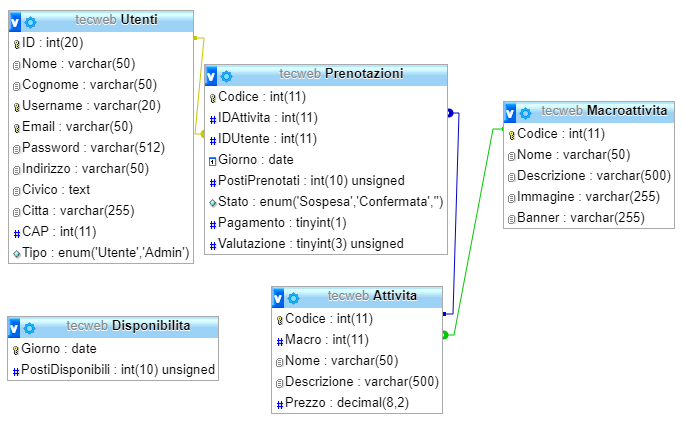
\includegraphics[scale=0.7]{images/erdb.png}}
\end{figure}
il database è inoltre privo di trigger, si è deciso infatti di gestire tramite PHP le varie operazioni riguardanti la gestione dei dati.
\subsection{Caricamento delle immagini}
**come abbiamo gestito il caricamento delle immagini per una nuova macroattività**